\chapter{未來研究建議}
本專題以虛實整合為出發點,將實體現有的3D列印機系統,透過虛擬環境來架設3D列印機,實現模擬現實列印的情況,並透過虛擬場景組裝uArm手臂,過程中使用pySTL來輔助CAD軟體的使用,繪製完的零件可以透過python程式達到輕易地更改stl檔的位置與大小,無須再打開CAD軟體操作,後續研究若是繼續往虛擬環境發展,可以研究xml使組合件的物體的位置標準化,往後零件尺寸有更改後無須再虛擬環境再重新組裝,虛擬場景裡就能自動組裝完,透過這項功能,使未來客製化的產品,都能輕易地在虛擬場景完成。 \\
\begin{figure}[hbt!]
\begin{center}
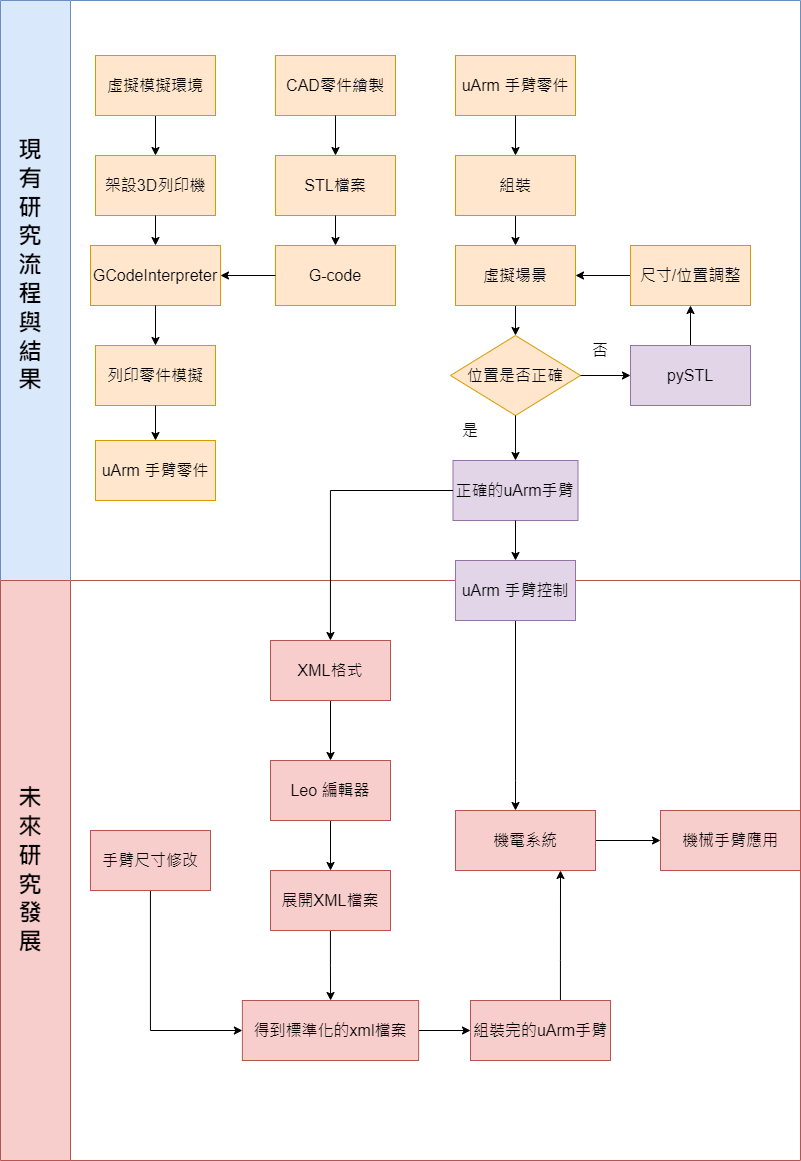
\includegraphics[width=16cm]{未來研究發展}
\caption{\Large 未來研究發展}
\label{未來研究發展}
\end{figure}
